\chapter{Analysis and Specifications}
\label{chap:Analysis_and_Specifications}

\section*{Introduction}
This chapter is dedicated to defining the detailed specifications and requirements of the proposed LegalTech platform. A thorough analysis is essential to ensure the system aligns with the project’s objectives and end-user expectations. In the following sections, we will categorize these specifications into functional requirements, detailing what the system must do; non-functional requirements, defining how the system should perform; and finally, the system constraints that set the boundaries for development, budget, and technology.

\newpage

\section{Functional Requirements}
This section outlines the functional requirements for the reusable architecture. These are the key
features and behaviors the architecture must support to facilitate the development of various GenAI-powered web applications.

\subsection{User Interface (UI)}
\begin{itemize}
    \item \textbf{Landing Page:} The platform shall provide an intuitive landing page that clearly explains the application's core concept, value proposition, and functionalities to the users.
    \item \textbf{Account Creation \& Login:} Users must be able to create an account and authenticate using multiple methods, including Email/Password, Google, Facebook, and Apple ID.
    \item \textbf{AI Chat Interface:} A dedicated chat page where the user can interact directly with the Large Language Model (LLM) powered by the RAG pipeline.
    \item \textbf{File Upload \& Management:} Users can upload their personal documents into the chat. Alternatively, they can store documents in a personal cloud space on the platform and import them into the chat whenever needed.
    \item \textbf{Document Generation:} Users shall be able to draft formal legal documents using LaTeX via direct code input.
    \item \textbf{AI-Assisted Drafting:} Users can prompt the Chatbot to automatically write, format, or modify legal documents based on pre-existing templates available on the platform.
\end{itemize}

\subsection{Large Language Model (LLM) Integration}
\begin{itemize}
    \item \textbf{Model Selection:} The platform must integrate a highly capable LLM suitable for complex legal reasoning.
    \item \textbf{Context Memory:} The LLM must retain the context of the conversation, remembering previous prompts and uploaded documents within the same session.
    \item \textbf{Role Prompting:} The LLM must be strictly guided by an engineered system prompt, enforcing specific rules and constraints to ensure it consistently maintains its designated role as a Moroccan legal assistant.
\end{itemize}

\subsection{Data Retrieval (RAG System)}
\begin{itemize}
    \item \textbf{RAG Architecture:} A Retrieval-Augmented Generation pattern shall be implemented to combine LLM-generated content with highly relevant factual data extracted from the document database.
    \item \textbf{Standardized Retrieval Mechanism:} The system shall utilize Vector Stores (Vector Databases) to ensure rapid, efficient, and semantically accurate search and retrieval of documents based on user queries.
\end{itemize}

\subsection{Authentication and Authorization}
\begin{itemize}
    \item \textbf{Multi-Provider Auth:} The system must implement robust authentication integrating third-party OAuth providers (Google, Facebook, Apple).
    \item \textbf{Admin Dashboard:} A secure, restricted-access dashboard must be available exclusively to administrators for user management and system monitoring.
\end{itemize}

\subsection{System Monitoring and Reporting}
\begin{itemize}
    \item \textbf{Smart Logging System:} An automated logging mechanism must be implemented. To optimize memory usage, logs will be compressed into \texttt{.gz} files at the end of each day and permanently deleted every 30 days.
    \item \textbf{Automated API Retry Mechanism:} To minimize error rates and ensure high availability, the server must automatically retry failed API requests multiple times before returning an error to the user.
\end{itemize}


\section{Non-Functional Requirements}
This section outlines the non-functional requirements that define how the architecture should perform,
focusing on critical attributes such as performance, scalability, and security.

\subsection{Performance}
\begin{itemize}
    \item \textbf{Concurrency:} The application must be capable of handling up to 100 concurrent users without degradation in service quality.
    \item \textbf{Response Time:} The system must deliver a response time of less than 120 seconds for queries.
    \item \textbf{Input Handling:} The architecture must efficiently process large input sizes (e.g., user prompts or document text up to 10,000 characters) without significant performance drops.
\end{itemize}

\subsection{Scalability}
\begin{itemize}
    \item \textbf{Horizontal Scaling:} The architecture shall be highly scalable, allowing the application to increase its capacity dynamically by adding more instances of core components, such as backend services, vector databases, and LLM API endpoints.
\end{itemize}

\subsection{Security}
\begin{itemize}
    \item \textbf{Data Protection:} The platform must implement industry-standard encryption and security protocols for user authentication and data storage.
    \item \textbf{Vulnerability Mitigation:} The application infrastructure must be strictly protected against common web vulnerabilities, specifically Distributed Denial of Service (DDoS) attacks and SQL Injection.
\end{itemize}


\section{System Constraints}
Constraints define the limitations and mandatory boundaries within which the project must be developed and operated.

\subsection{Budget Constraints}
\begin{itemize}
    \item \textbf{Cost Optimization:} Applications built using this architecture must be highly optimized for cost efficiency to minimize long-term operational costs (e.g., API usage, cloud hosting).
    \item \textbf{Flexible Deployment:} The architecture must support flexible deployment options to allow migration to more cost-effective hosting providers if necessary.
\end{itemize}

\subsection{Time Constraints}
\begin{itemize}
    \item \textbf{Development Timeline:} While the reusable architecture is designed to be adaptable, the complete development, testing, and deployment of this specific application must strictly fall within a 3-month project timeline.
\end{itemize}

\subsection{Technological Constraints}
\begin{itemize}
    \item \textbf{Pre-Approved Tech Stack:} The architecture must strictly adhere to a pre-approved technology stack. This includes using \textbf{Python} for all backend services and AI pipelines, and \textbf{React} for frontend development.
    \item \textbf{Stack Deviations:} Any deviation from or addition to the core technology stack must be fully justified and formally approved by the stakeholders managing the architecture's governance.
\end{itemize}


\section{System Modeling (UML)}
\subsection{Use Case}
Un acteur spécifie un rôle joué par un utilisateur ou tout autre système qui interagit avec le sujet. Il peut représenter des rôles joués par des utilisateurs humains, du matériel externe ou d’autres sujets. Les acteurs sont toujours en dehors du système et interagissent directement avec lui en initiant un cas d’utilisation, en lui fournissant des entrées et/ou en recevant des sorties.

Dans notre plateforme, on a 3 acteurs qui peuvent y accéder :

\subsubsection*{Human Actors}
\begin{itemize}
    \item \textbf{User:} The primary end-user of the platform. This actor can manage their account, interact with the AI chatbot, upload and edit legal documents, and compile templates into final PDF files.
    \item \textbf{Administrator:} A privileged user responsible for the overall governance of the platform. They have the authority to oversee, control, and manage all registered users and their access rights.
    \item \textbf{Log Responsible:} A specialized technical actor dedicated to system maintenance. They are responsible for monitoring system logs, tracking errors, and managing data retention to ensure platform stability.
\end{itemize}

\subsubsection*{External Systems (External Actors)}
\begin{itemize}
    \item \textbf{Clerk Auth:} An external Identity and Access Management (IAM) provider utilized by the platform to securely handle user registration, login, and session management.
    \item \textbf{Gemini LLM:} The external Large Language Model API that powers the conversational capabilities of the platform, providing context-aware legal reasoning and text generation within the chat.
    \item \textbf{GPT-4o OCR:} An external AI-driven Vision model integrated to perform advanced Optical Character Recognition, extracting text and tables from complex scanned documents uploaded by the user.
    \item \textbf{LaTeXLite:} An external compilation engine service used by the workspace to seamlessly convert user-generated LaTeX code and templates into properly formatted PDF documents.
\end{itemize}

\subsection{Use Case Diagrams}
\begin{figure}[htbp]
    \centering
    \IfFileExists{Figures/use_case.png}{
        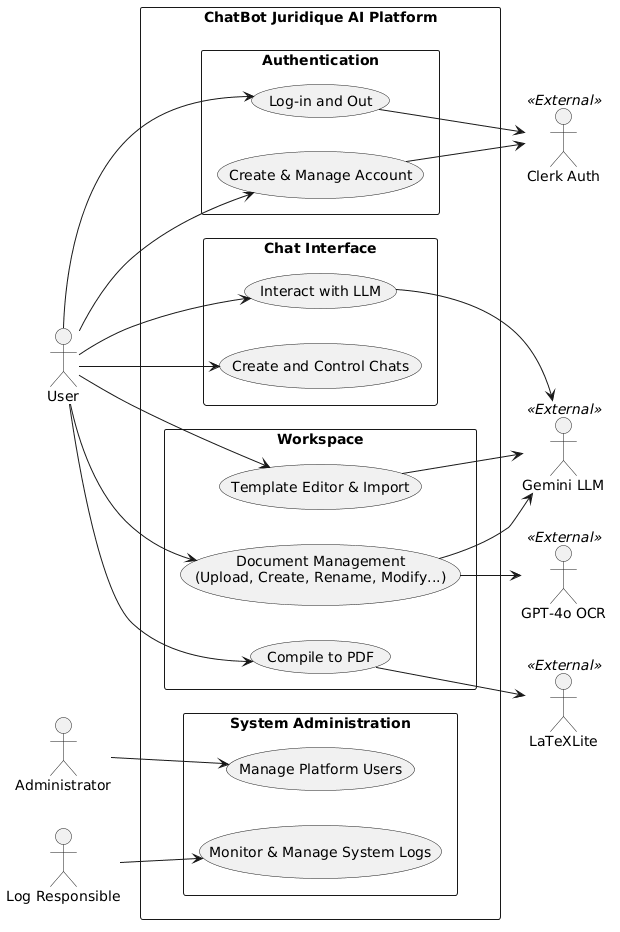
\includegraphics[width=0.4\textwidth]{Figures/use_case.png}
    }{
        \framebox[10cm]{\rule{0pt}{8cm} \textbf{Image manquante: Figures/use_case.png (Use Case Diagram)}}
    }
    \caption{Global Use Case Diagram of the ChatBot Juridique AI Platform}
    \label{fig:use_case_diagram}
\end{figure}

\newpage

\section{System Behavior (Sequence Diagrams)}

Sequence diagrams are essential for visualizing the dynamic behavior of the system. They detail how different components, APIs, and external services interact over time to execute the core functionalities of the platform.

\subsection{Chat Management and Live File Upload}
This sequence diagram comprehensively details the lifecycle of a chat session. It illustrates how a user creates a new session, optionally uploads a live file (triggering a multimodal prompt bypass), sends prompts that interact with the RAG pipeline, and manages the chat metadata (such as renaming or pinning the conversation) through the FastAPI backend and PostgreSQL database.

\begin{figure}[H]
    \centering
    \IfFileExists{Figures/seq_chat_management.png}{
        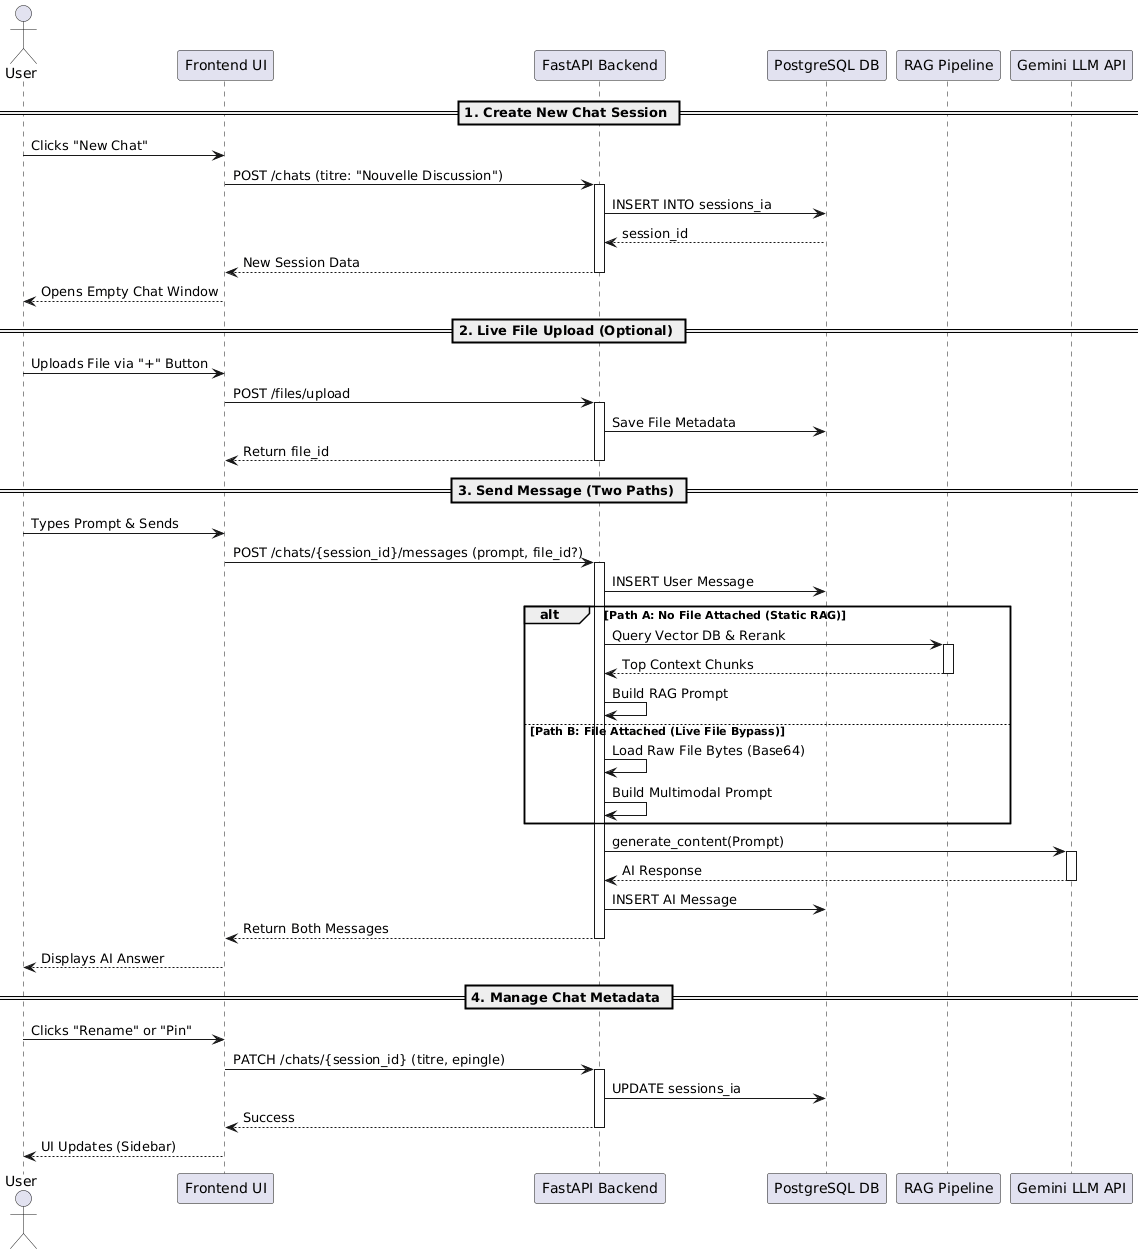
\includegraphics[width=0.7\textwidth]{Figures/seq_chat_management.png}
    }{
        \framebox[14cm]{\rule{0pt}{7cm} \textbf{Image manquante: Figures/seq_chat_management.png}}
    }
    \caption{Sequence Diagram of Chat Session Management and Multimodal Interaction}
    \label{fig:seq_chat_management}
\end{figure}

\newpage

\subsection{Core RAG Pipeline Execution}
This diagram maps the core query execution process when a user asks a legal question. It highlights the journey of the user's prompt as it is embedded, retrieved via semantic search in ChromaDB, reranked for maximum relevance, and finally sent to the Gemini LLM to generate a grounded response.

\begin{figure}[H]
    \centering
    \IfFileExists{Figures/seq_rag_pipeline.png}{
        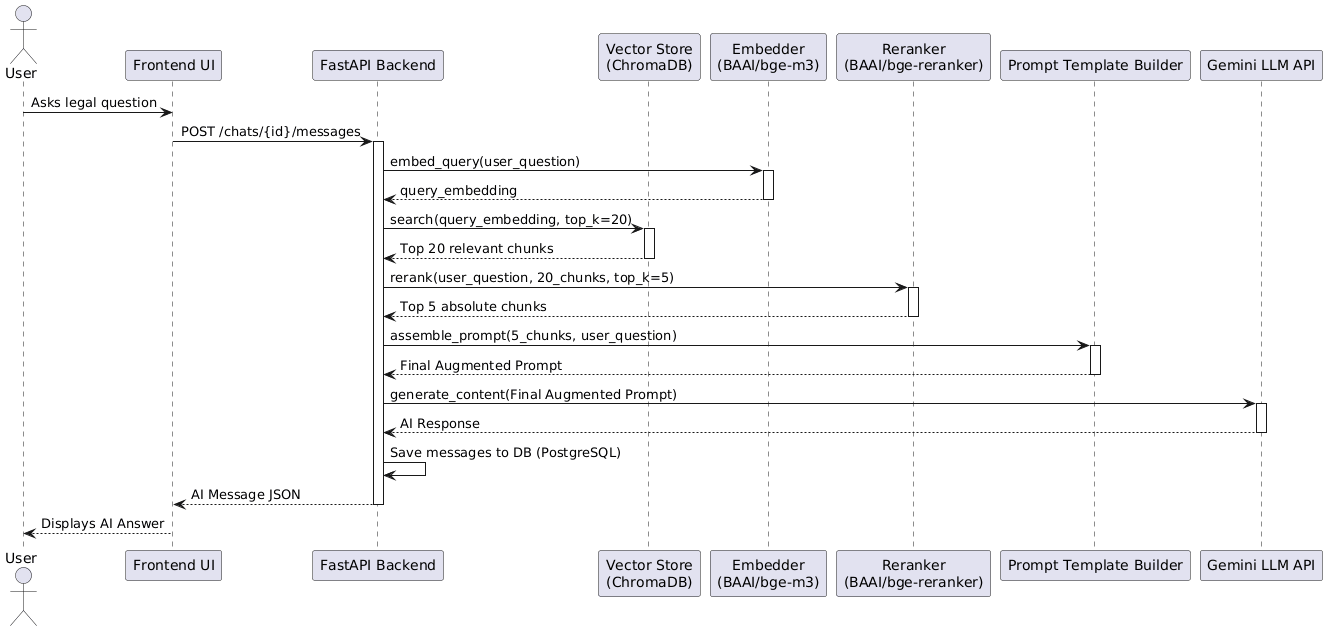
\includegraphics[width=1\textwidth]{Figures/seq_rag_pipeline.png}
    }{
        \framebox[14cm]{\rule{0pt}{7cm} \textbf{Image manquante: Figures/seq_rag_pipeline.png}}
    }
    \caption{Sequence Diagram of the Retrieval-Augmented Generation (RAG) Pipeline}
    \label{fig:seq_rag}
\end{figure}

\newpage

\subsection{Document Upload and Data Ingestion}
This workflow details the complex data ingestion process for Moroccan legal documents. It demonstrates how raw PDFs are converted into images, processed by the GPT-4o Vision OCR to filter visual noise and extract Markdown tables, semantically chunked, and indexed into the vector database.

\begin{figure}[H]
    \centering
    \IfFileExists{Figures/seq_doc_upload.png}{
        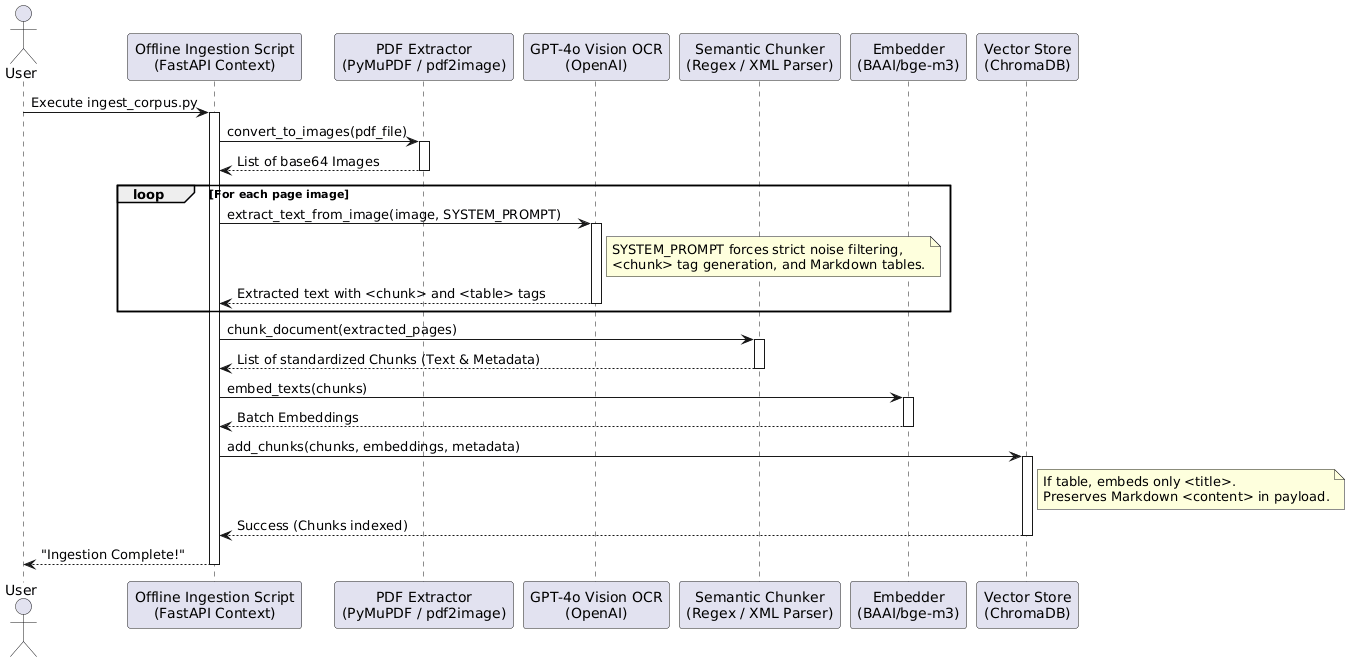
\includegraphics[width=1\textwidth]{Figures/seq_doc_upload.png}
    }{
        \framebox[14cm]{\rule{0pt}{7cm} \textbf{Image manquante: Figures/seq_doc_upload.png}}
    }
    \caption{Sequence Diagram of the Document Upload and OCR Ingestion Process}
    \label{fig:seq_upload}
\end{figure}

\vspace{1cm}

\subsection{AI-Assisted Document Generation}
This sequence diagram illustrates the LaTeX document drafting and compilation feature. It describes how user commands trigger template retrieval, which the LLM then adapts into valid LaTeX code, followed by a compilation request (using pdfLaTeX or LaTeXLite) to render the final PDF document for the user.

\begin{figure}[H]
    \centering
    \IfFileExists{Figures/seq_doc_generation.png}{
        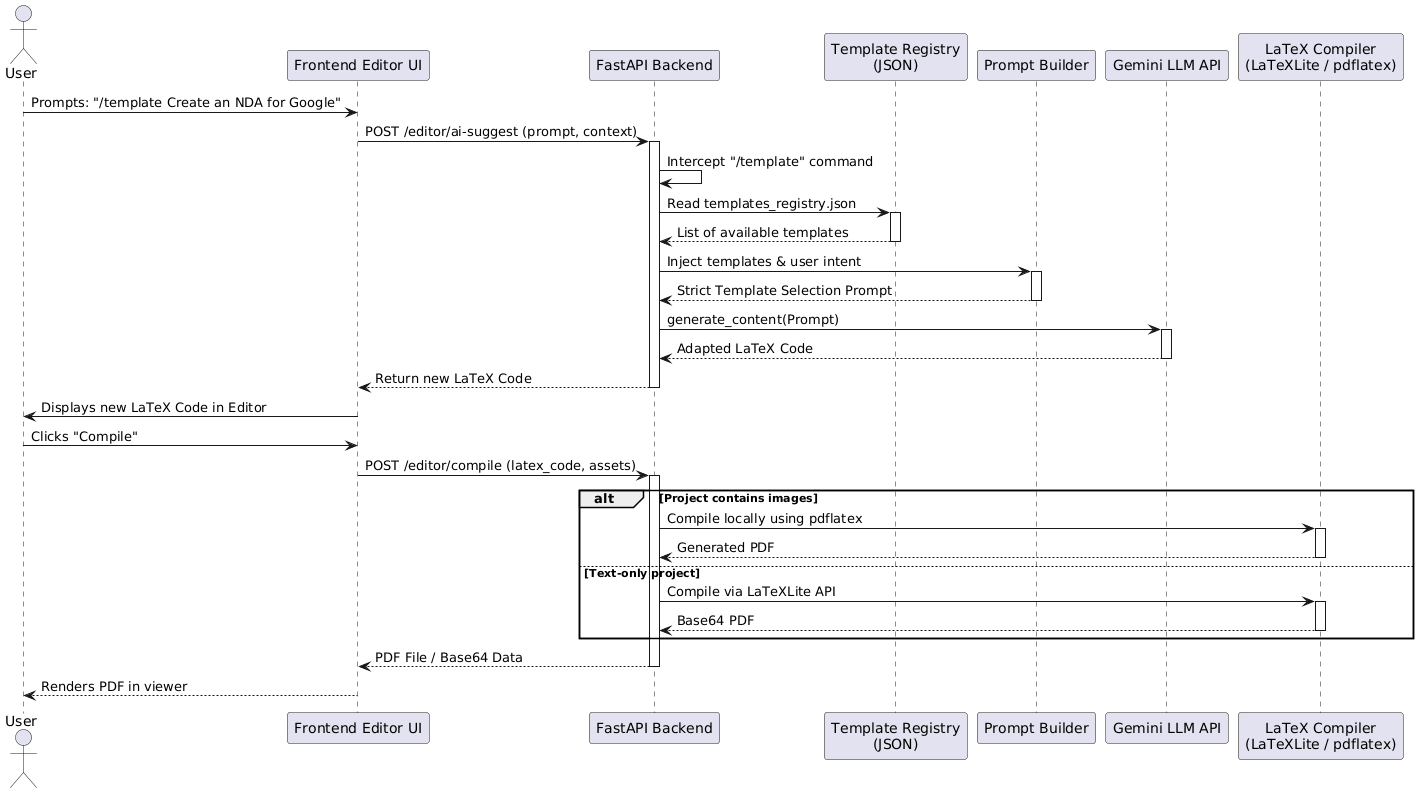
\includegraphics[width=1\textwidth]{Figures/seq_doc_generation.png}
    }{
        \framebox[14cm]{\rule{0pt}{7cm} \textbf{Image manquante: Figures/seq_doc_generation.png}}
    }
    \caption{Sequence Diagram of the AI-Assisted Document Generation and Compilation}
    \label{fig:seq_generation}
\end{figure}
\newpage
\section{Database Architecture and Optimization}

\subsection{Class Diagram (Entity-Relationship Model)}
The Class Diagram serves as the foundational blueprint for our PostgreSQL database. It illustrates the core entities—such as Users, Chat Sessions, Messages, and Documents—along with their attributes, primary keys, foreign keys, and relational multiplicities. This ensures a robust, normalized, and scalable data structure.

\begin{figure}[H]
    \centering
    \IfFileExists{Figures/class_database.png}{
        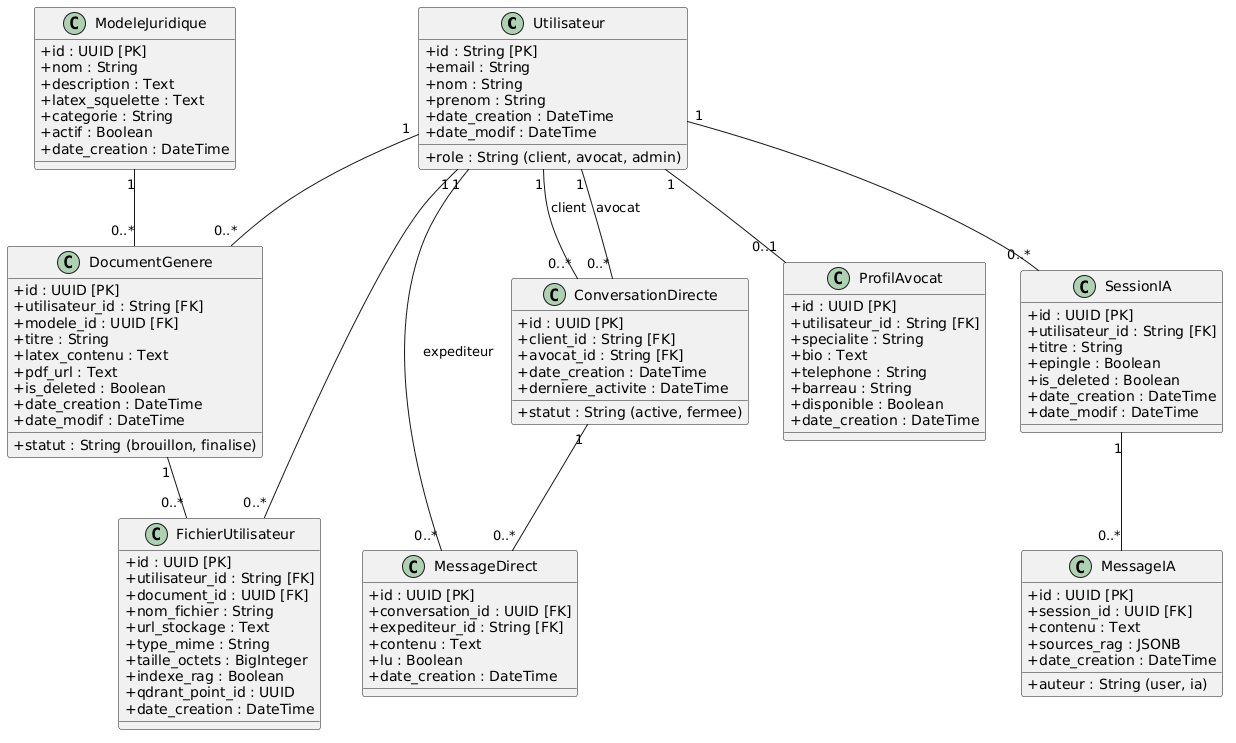
\includegraphics[width=1\textwidth]{Figures/class_database.png}
    }{
        \framebox[14cm]{\rule{0pt}{7cm} \textbf{Image manquante: Figures/class_database.png}}
    }
    \caption{UML Class Diagram representing the PostgreSQL Database Schema}
    \label{fig:class_diagram}
\end{figure}

\subsection{Database Optimization Strategies}
To ensure high performance, data integrity, and secure tenant isolation, we implemented advanced structural optimizations directly within the PostgreSQL engine.

\begin{itemize}
    \item \textbf{Advanced Indexing Strategies:} To minimize latency on high-volume queries, some indexes:
    \begin{itemize}
        \item \textit{Partial \& Compound Indexes:} Created \texttt{idx\_sessions\_active} to index only active sessions and pre-sort by \texttt{date\_modif DESC} for instant UI loading.
        \item \textit{Foreign Key Indexing:} Explicitly indexed all foreign keys to prevent full-table scans during heavy \texttt{JOIN}s.
        \item \textit{GIN Indexing:} Applied GIN indexes to RAG metadata for rapid semantic searches without payload deserialization.
    \end{itemize}
    
    \item \textbf{PL/pgSQL Triggers \& Automation:} A custom PL/pgSQL function and \texttt{BEFORE UPDATE} triggers automatically manage timestamps (e.g., setting \texttt{date\_modif} to \texttt{now()}), ensuring chronological integrity and reducing application-layer logic.
    
    \item \textbf{Data Integrity \& Constraints:} Strict relational rules prevent orphaned data and corrupted states:
    \begin{itemize}
        \item \textit{Cascading Deletes (\texttt{ON DELETE CASCADE}):} Child tables are strictly bound to parent IDs, ensuring clean deletions in a single transaction.
        \item \textit{Check Constraints (\texttt{CHECK}):} Constrained vocabularies (e.g., user roles) are enforced directly on columns to reject malformed strings.
    \end{itemize}
    
    \item \textbf{Aggregated Views:} A materialized SQL VIEW (\texttt{v\_dashboard\_utilisateur}) pre-calculates complex aggregations (session counts, documents, RAG files) in a single pass. This enables instant analytics retrieval for the Dashboard API without expensive real-time \texttt{COUNT} operations.
\end{itemize}
\section*{Conclusion}
In conclusion, this chapter has established a comprehensive blueprint for the project by detailing the functional, non-functional, and systemic requirements. By explicitly outlining the user interface features, RAG and LLM integrations, performance benchmarks, and strict security and budgetary constraints, we have defined the exact criteria for a successful implementation. These specifications will serve as the guiding reference for the architectural design and software development phases discussed in the subsequent chapters.

\pagebreak